\documentclass[review]{elsarticle}

\usepackage{lineno,hyperref}
\modulolinenumbers[5]

\journal{Journal of \LaTeX\ Templates}

%%%%%%%%%%%%%%%%%%%%%%%
%% Elsevier bibliography styles
%%%%%%%%%%%%%%%%%%%%%%%
%% To change the style, put a % in front of the second line of the current style and
%% remove the % from the second line of the style you would like to use.
%%%%%%%%%%%%%%%%%%%%%%%

%% Numbered
%\bibliographystyle{model1-num-names}

%% Numbered without titles
%\bibliographystyle{model1a-num-names}

%% Harvard
%\bibliographystyle{model2-names.bst}\biboptions{authoryear}

%% Vancouver numbered
%\usepackage{numcompress}\bibliographystyle{model3-num-names}

%% Vancouver name/year
\usepackage{numcompress}\bibliographystyle{model4-names}\biboptions{authoryear}

%% APA style
%\bibliographystyle{model5-names}\biboptions{authoryear}

%% AMA style
%\usepackage{numcompress}\bibliographystyle{model6-num-names}

%% `Elsevier LaTeX' style
\bibliographystyle{elsarticle-num}
%%%%%%%%%%%%%%%%%%%%%%%

\graphicspath{{./figure/}}

\usepackage{amsmath}
\usepackage{amssymb}
\usepackage{xeCJK}
\usepackage{enumerate}
\usepackage{amsthm}
\newtheorem{theorem}{Theorem}
\newtheorem{corollary}[theorem]{Corollary}
\newtheorem{lemma}{Lemma}
\newtheorem{example}{Example}
\newtheorem{proofOfTheorem}{Proof of Theorem}
\begin{document}

\begin{frontmatter}

\title{积分似然比检验\tnoteref{mytitlenote}}
\tnotetext[mytitlenote]{Fully documented templates are available in the elsarticle package on \href{http://www.ctan.org/tex-archive/macros/latex/contrib/elsarticle}{CTAN}.}

%% Group authors per affiliation:
\author{author \fnref{myfootnote}}
\address{Radarweg 29, Amsterdam}
\fntext[myfootnote]{Since 1880.}

%% or include affiliations in footnotes:
\author[mymainaddress,mysecondaryaddress]{Elsevier Inc}
\ead[url]{www.elsevier.com}

\author[mysecondaryaddress]{Global Customer Service\corref{mycorrespondingauthor}}
\cortext[mycorrespondingauthor]{Corresponding author}
\ead{support@elsevier.com}

\address[mymainaddress]{1600 John F Kennedy Boulevard, Philadelphia}
\address[mysecondaryaddress]{360 Park Avenue South, New York}

\begin{abstract}
    本文针对一般的检验问题,提出了积分似然比检验方法,得到了其在原假设下的分布和局部功效函数,并在较弱的条件下给出了严格证明。我们的定理可以适用于似然函数有界的情形,由于此时似然比检验不存在,所以理论上积分似然比检验可以解决一些似然比检验无法解决的问题。而实际上,混合正态模型正好是这样的例子,积分似然比检验水平控制的很好,而对应的,似然比统计量甚至不存在。在我们的定理无法应用的情形,比如高维情形,积分似然比方法仍然是一种寻找检验的优良方法。我们考虑了高维均值检验问题,此时似然比检验不存在,而积分似然比方法依然存在,所以可以作为似然比检验在高维情形下的一种替代品,它具有类似似然比检验的优良性质,模拟结果显示在一些情形下,它优于已有的检验方法。
\end{abstract}

\begin{keyword}
\texttt{elsarticle.cls}\sep \LaTeX\sep Elsevier \sep template
\MSC[2010] 00-01\sep  99-00
\end{keyword}

\end{frontmatter}

\linenumbers

\section{介绍}

 \cite{Aitkin1991Posterior}针对检验问题$H_0:\theta\in \Theta_0$ vs $H_1:\theta\in \Theta_1$提出了后验贝叶斯因子,形式是
\begin{equation}
    \frac{\int_{\Theta} p(X|\theta)\pi(\theta|X)\, d\theta}{\int_{\Theta_0}p(X|\theta)\pi^*(\theta|X)\, d\theta}
\end{equation}
其中$X=X_1,\cdots,X_n$是观测数据, $p(x|\theta)$是样本密度, $\pi^*(\theta|x)$是原假设下的后验密度,$\pi(\theta|x)$是被择假设下的后验密度。
\cite{gelfand1993bayesian}利用了拉普拉斯近似求得了它在原假设的分布。他们的方法并没有显式的给出定理成立需要的条件,而且证明依赖于拉普拉斯近似,这就假设了极大似然估计的存在。而当极大似然估计存在时,似然比检验也存在。所以他们的结论并没有显示出后验贝叶斯因子比似然比检验更为广泛的适用性。

基于后验贝叶斯因子,我们考虑更一般的积分似然比检验统计量:
\begin{equation}
    \Lambda (X)=\frac{\int_{\Theta} p(X|\theta)\pi(\theta;X)\,d\theta}{\int_{\Theta_0} p(X|\theta)\pi^*(\theta;X)\,d\theta}
\end{equation}
其中$\pi(\theta;X)$和$\pi^*(\theta;X)$是基于数据的权函数,但不必等于后验密度。

似然比检验是被最广泛使用的统计方法,它具有很多最优性质,比如由NP引理,它在简单原假设和简单被择假设下是最有效检验,见\cite{Lehmann}。在多维情形,一般是没有最有效检验的,但是似然比检验是在Bahadur efficiency的意义下是渐进最优的,见\cite{MR0315820}。而我们知道在许多模型中,即使是一些被广泛使用的模型,似然也经常是是无界的,见\cite{Cam1990Maximum}。这种情形下,似然比检验不存在。但此时积分似然比检验是可能存在的,比如后面我们举的例子。

参考Bernstein-von Mises定理的证明,见\cite{van2000asymptotic},本文在很一般的假设下证明积分似然比检验的Wilks现象及局部功效,尤其是我们的定理不要求似然函数有界,这使得我们的方法可以用于一些似然无界在的模型。并举例说明其广泛的适用性。

\section{Integrated likelihood ratio test}

Let $X_1,\cdots,X_n$ be a sample from $P_{\theta}, \theta\in\Theta$. Denote $X=(X_1,\cdots,X_n)$. The parameter space $\Theta$ is an open subset of $\mathbb{R}^{p_2}$. The null space $\Theta_0$ is a $p_1$-dimensional subspace of $\Theta$
\begin{equation}
    \Theta_0=\{\theta\in\Theta:\theta_{p_1+1}=\theta_{0,{p_1+1}},\cdots,\theta_{p_2}=\theta_{0,{p_2}}\},
\end{equation}
where the last $p_2-p_1$ parameters $\theta_{0,{p_1+1}},\cdots,\theta_{0,{p_2}}$ are fixed. We want to test the hypotheses
\begin{equation}
H_0:\theta\in \Theta_0\quad vs. \quad H_1:\theta\in \Theta.
\end{equation}
The first $p_1$ parameters are nuisanse parameters.

$\Theta_0$ can be regarded as a open subset of $\mathbb{R}^{p_1}$. To simplifies notations, we denote  $\Theta^*_0=\{(\theta_1,\cdots,\theta_{p_1})^T:\, (\theta_1,\cdots,\theta_{p_1},\theta_{0,p_1+1},\theta_{0,p_2})\in \Theta_0\}$. And we could use $p_1$-dimensional vector $\theta^*\in
\Theta_0^*$ to represent $\theta\in\Theta_0$ and regard $\Theta_0^*$ as null space.  Let $\pi(\theta;X)$ and $\pi^*(\theta^*;X)$ be the weight functions in $\Theta$ and $\Theta_0^*$. The integrated likelihood ratio statisitc is defined as
\begin{equation}\label{likelihoodRatio}
    \Lambda (X)=\frac{\int_{\Theta} p(X|\theta)\pi(\theta;X)\,d\theta}{\int_{\Theta^*_0} p(X|\theta^*)\pi^*(\theta^*;X)\,d\theta^*}
\end{equation}


\section{Main results}

We will denote by $\rightsquigarrow$ the weak convergence. 
$dN(\mu,\Sigma)(h)$ is the density function of a normal distribution with mean $\mu$ and variance $\Sigma$.

Assume $\theta_0\in\Theta_0$ is a fixed parameter in null space. We study the asymptotic behavior of integrated likelihood ratio statistic around $\theta_0$.
设试验$P_\theta : \theta\in \Theta$在$\theta_0$处均方可微,即存在随机$\dot{\ell}_{\theta_0}$使得
\begin{equation}
    \int \big[\sqrt{p_{\theta_0+h}}-\sqrt{p_{\theta_0}}-\frac{1}{2}h^T\dot{\ell}_{\theta_0}\sqrt{p_{\theta_0}}\big]^2\, d\mu=o(\|h\|^2),\quad h\to 0
\end{equation}
其中$\mu$是$P_{\theta}$的控制测度。而$p_{\theta}(x)$是$P_{\theta}(x)$相对于$\mu$的密度函数。$\dot{\ell}_{\theta_0}$是均方可微意义下的得分函数。

设$I_{\theta_0}=P_{\theta_0}\dot{\ell}_{\theta_0}\dot{\ell}_{\theta_0}^T$是$\theta_0$处均方可微意义下的信息阵,
设“局部充分统计量”$\Delta_{n,\theta_0}=\frac{1}{\sqrt{n}}\sum_{i=1}^n I_{\theta_0}^{-1}\dot{\ell}_{\theta_0}(X_i)$。相对应的,在原空间中$\dot{\ell}^*$,$I^*_{\theta_0}$,$\Delta_{n,\theta_0}^*$均可同样定义。我们很容易知道,$\dot{\ell}^*_{\theta_0}$是$\dot{\ell}_{\theta_0}$的前$p_1$维向量,$I^*_{\theta_0}$是$I_{\theta_0}$左上角的$p_1\times p_1$维矩阵,$\Delta_{n,\theta_0}^*=\frac{1}{\sqrt{n}}\sum_{i=1}^n I_{\theta_0}^{*-1}\dot{\ell}^*_{\theta_0}(X_i)$

Let $h=\sqrt{n}(\theta-\theta_0)$ which reparameterize   $\theta$ around $\theta_0$ by the scale of $\sqrt{n}$.  Obviously, $h=0$ under null. Under local alternatives, $h$ is assumed to converge to a constant.

Listed below are the regular conditions we need:

\begin{enumerate}[(i)]
    \item
        设Bernstein-von Mises定理(见\cite{van2000asymptotic})的条件满足: $\Theta$是$\mathbb{R}^p$的开子集,试验($P_{\theta}:\theta\in\Theta$)在$\theta_0\in \Theta$处均方可微,具有非奇异信息阵$I_{\theta_0}$,假设对任意的$\epsilon>0$,存在一个相合检验序列:
        \begin{equation}
            P_{\theta_0}^n\phi_n\to 0,\quad \sup_{\|\theta-\theta_0\|\geq \epsilon} P_\theta^n(1-\phi_n)\to 0.
        \end{equation}
        设$\pi_n(h;X)$是一个满足Bernstain-von Mises定理结论的权函数:
        \begin{equation}
            \|\pi_n(h;X)-dN(\Delta_{n,\theta_0},I_{\theta_0}^{-1})(h)\|\overset{P_{\theta_0}^n}{\to}0
        \end{equation}
    \item
        $\pi_n(h;X)$的支撑在$\|h\|\leq K\sqrt{n}$上,$K$是一个固定常数。$\sup_h |\pi_n(h;X)|\leq A$对某个$A$依概率成立。
    \item
        存在$\theta_0$的某个邻域$V$和某个函数$\dot{\ell}$满足$P_{\theta_0}\dot{\ell}^2<\infty$,对$\forall \theta_1,\theta_2\in V$,有
        \begin{equation}
            |\log p_{\theta_1}(x)-\log p_{\theta_2}(x)|\leq \dot{\ell}(x)\|\theta_1-\theta_2\|.
        \end{equation}
\end{enumerate}

条件$(i)$是很弱的条件。条件(ii)中的支撑条件可以等价的表述为$\pi_n(h;X)$作为$\theta$的函数,其支撑有界。对于一个统计模型,我们通常认为似然函数在很远处的取值没有太大意义,所以不分配权是合理的。因为我们不该某个$\theta$附近分配过大的权,所以权函数有界的条件也是合理的。事实上,我们总可以把后验密度$\pi_n(h|X)$改造成满足条件$(ii)$的权函数$\pi_n(h;X)$,比如我们选取一个充分大的$M$,则容易证明
\begin{equation}
    \pi_n(h;X)=\min(\pi_n(h|X),M) 1_{\|h\|\leq K\sqrt{n}}
\end{equation}
同时满足条件$(i)$,$(ii)$。而且我们有理由相信这样得到的权函数比后验密度收敛的更快一点。
均方可微条件使得似然可以在$\theta_0$的邻域内展开,我们在证明一般性的定理时需要把似然函数在$\theta_0$的邻域内一致展开,所以我们需要条件$(iii)$。

我们的第一个定理是
\begin{theorem}\label{theoremMain}
    如果条件$(i)$,$(ii)$,$(iii)$满足,设$\eta_n$是有界实数序列,那么我们有
%    \begin{equation}
%        \Big|\int_{\mathbb{R}^{p}}\frac{p_h(X)}{p_0(X)}\pi_n(h;X)\,dh-\int_{\mathbb{R}^{p}}e^{h^TI_{\theta_0}\Delta_{n,\theta_0}-\frac{1}{2}h^TI_{\theta_0}h}dN(\Delta_{n,\theta_0},I_{\theta_0}^{-1})(h)\,dh\Big|\xrightarrow{P_{\eta_n}^n}0
%    \end{equation}
    \begin{equation}
        \Big|\int_{\mathbb{R}^{p}}\frac{p_h(X)}{p_0(X)}\pi_n(h;X)\,dh-
        2^{-\frac{p}{2}}e^{\frac{1}{2}\Delta_{n,\theta_0}^TI_{\theta_0}\Delta_{n,\theta_0}}
        \Big|\xrightarrow{P_{\eta_n}^n}0
    \end{equation}
\end{theorem}
基于定理\ref{theoremMain},我们可以得到积分似然比统计量在原假设的渐进分布,也就是wilks现象。我们可以根据此渐进分布来决定检验的临界值
\begin{theorem}\label{theoremWilks}
    设定理\ref{theoremMain}的条件对原空间$\Theta_0$和全空间$\Theta$均成立,真实参数$\theta_0$是$\Theta$的一个内点,同时是$\Theta_0$的一个相对内点,那么我们有
\begin{equation}
    2\log(\Lambda(X))\overset{P_0^n}{\rightsquigarrow} \chi^2_{p_2-p_1}-(p_2-p_1)\log(2)
\end{equation}

\end{theorem}


有了定理\ref{theoremMain},我们可以利用Le Cam第三引理得到积分似然比统计量在局部被择下的渐近分布:
\begin{theorem}   \label{theoremPower}
    设定理\ref{theoremMain}的条件对原空间$\Theta_0$和全空间$\Theta$均成立。$\theta_0$是$\Theta_0$的一个内点,同时是$\Theta_0$的一个相对内点。真实参数$\theta$满足$\eta_n=\sqrt{n}(\theta-\theta_0)\to \eta$。若
\begin{equation}
    I_{\theta_0}=\left(
        \begin{matrix}
            I^*_{\theta_0}&I_{12}
            \\
            I_{21}&I_{22}
        \end{matrix}
    \right)
\end{equation}
$I_{22\cdot 1}=I_{22}-I_{21}I_{\theta_0}^{*-1}I_{12}$
    那么我们有
\begin{equation}
    2\log(\Lambda(X))\overset{P_0^n}{\rightsquigarrow} \chi^2_{p_2-p_1}(\delta)-(p_2-p_1)\log(2)
\end{equation}
其中
\begin{equation}
\delta=\eta^T
    \left(
        \begin{matrix}
            0&0\\
            0&I_{22\cdot 1}
        \end{matrix}
    \right)
    \eta
\end{equation}
\end{theorem}

我们的结果和似然比检验结果很类似。这样的结果可以从试验的收敛的观点来解释。从渐进的角度来讲,我们在$n$个样本空间中的统计问题近似于只观测到一个量$\Delta_{n,\theta_0}$。而在$h_n\to h$时,$\Delta_{n,\theta_0}\rightsquigarrow N(h,I_{\theta_0}^{-1})$。所以问题可以近似为只有一个观测$X\sim
N(h,I_{\theta_0}^{-1})$的问题。在这种情形下,我们可以直接计算似然比统计量,正是我们定理的结论。这样我们定理的结论就没什么奇怪的了。

\section{混合正态分布}
\cite{Cam1990Maximum}给出了一些似然无界的例子。混合正态分布是其中给出的第一个例子。这一节通过这个例子来说明积分似然比方法的优越性。

设$X_1,\cdots,X_n$ i.i.d. 服从混合正态分布
\begin{equation}
    \frac{1-\alpha}{\sqrt{2\pi}}\exp\left\{-\frac{1}{2}(x-\mu)^2\right\}+
    \frac{\alpha}{\sigma\sqrt{2\pi}}\exp\left\{-\frac{1}{2}\frac{(x-\mu)^2}{\sigma^2}\right\}
\end{equation}
其中$\alpha$是已知的固定参数。参数空间设为
\begin{equation}
    \Theta=\{\theta=(\mu,\sigma^2)^T:\mu\in(\-\infty,\infty),\sigma^2\in (0,M)\}
\end{equation}
\cite{Cam1990Maximum}指出,在这个模型下,似然函数是无界的。事实上,令$\mu=X_1$,然后令$\sigma^2\to 0$,则似然函数趋于无穷。

现在我们在这个模型下考虑检验问题$H_0:\mu=0,\sigma=2$ vs $H_1:\theta\in
\Theta$。似然比检验显然已经失效了,但此时积分似然比统计量仍然可以使用。事实上,我们可以验证(虽然很繁琐)条件$(i)$,$(ii)$,$(iii)$均成立,所以定理\ref{theoremWilks}和\ref{theoremPower}均成立。当然要想使用积分似然比统计量,我们需要寻找权函数,在这个例子中我们考虑用后验密度。这里我们可以看出,假设我们先验设置成无信息先验,那么后验密度与似然函数成正比,所以是无界的。无界的权函数不仅会使得我们的定理条件$(ii)$无法满足,更重要的是,在积分似然比统计量中,它会给似然函数在没意义的地方设置过多的权重,而我们实际上期望权函数集中在真实参数附近,所以无界的权函数使得统计量的性质变得很复杂并且收敛速度变慢。一种解决这个问题的方法是按照前面提到的,选取一个合适的充分大的$M^*$,定义新的权函数为
\begin{equation}
    \min(\pi_n(h;X),M^*)
\end{equation}
则新的有界的权函数依然满足条件$(i)$,甚至表现的更好。而条件$(ii)$也满足了。

在我们这个例子中,我们并不需要这样解决权函数无界的问题。因为我们只要设置合适的先验分布,后验密度就会有界,这样我们仍然可以使用后验密度作为权函数。我们发现当$\mu=X_1$, $\sigma^2\to 0$时,似然趋于无穷的速度正比例于$\frac{1}{\sigma}$。所以我们设置合适的先验对冲掉这个量。容易看出,$\chi^2(3)$的密度函数正好可以做到这一点。

故我们设先验是
\begin{equation}
    dN(0,1)(\mu)\times d\chi^2(3)(\sigma^2)
\end{equation}
其中$d\chi^2(3)(\sigma^2)$代表自由度为$3$的$\chi^2$分布的密度函数在$\sigma^2$处的取值。由于参数空间的限制,$\sigma^2$只在$(0,M)$上取值,所以这个先验并不是个概率密度,但这并不妨碍我们求得后验密度并计算积分似然比统计量。

我们下面通过数值模拟验证Wilks现象。我们取样本量$n=50,100,200$和超参数$\alpha=0.1,0.5,0.9$。每种情况重复抽取$1000$次样本,得到$1000$个积分似然比统计量。理想情况应该是它们的样本与$\chi^2(2)$的分布很接近。我们画出样本分布相对于$\chi^2(2)$分布的QQ图,模拟显示样本分布与$\chi^2(2)$分布很接近,见下图:

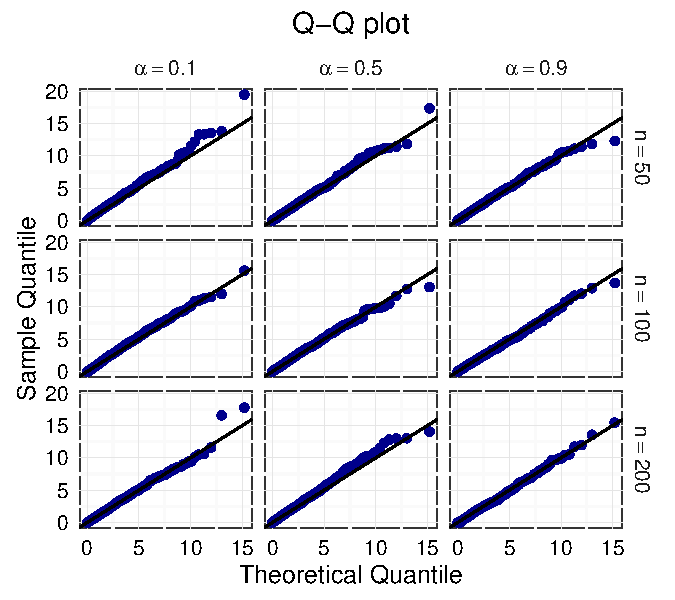
\includegraphics{myQQPlot.pdf}






\section{Appendix}
对于两个测度序列$P_n$和$Q_n$, $P_n\triangleleft \triangleright Q_n$代表$P_n$和$Q_n$是mutrally contiguous的,即对任意的随即变量序列$T_n$,有$T_n\overset{P_n}{\rightsquigarrow}0\Leftrightarrow T_n\overset{Q_n}{\rightsquigarrow}0$
\begin{lemma}\label{lemmaEx}
    假设$\Theta$是一个$\mathbb{R}^p$的一个开子集并且试验($P_\theta: \theta \in\Theta$)在$\theta_0$处均方可微。那么$P_{\theta_0}\dot{\ell}_{\theta_0}=0$,并且Fisher信息阵$I_{\theta_0}=P_{\theta_0}\dot{\ell}_{\theta_0}\dot{\ell}_{\theta_0}^T$存在。进一步,对于每个收敛序列$h_n\to h$,随着$n\to \infty$,有
    \begin{equation}
        \log \frac{p^n_{h_n}(X)}{p^n_0(X)}=\frac{1}{\sqrt{n}}\sum^n_{i=1}h^T\dot{\ell}_{\theta_0}(X_i)-\frac{1}{2}h^TI_{\theta_0}h+o_{P_{\theta_0}}(1)
    \end{equation}
    见\cite{van2000asymptotic}
\end{lemma}



\begin{lemma}\label{lemmaContiguity}
    设引理\ref{lemmaEx}条件满足。假设$T_n$是一个统计量序列,$U$是一个以原点为中心的球。则
    对任意的随机变量序列$T_n$, $T_n\overset{P^n_0}{\rightsquigarrow}0\Leftrightarrow T_n\overset{P^n_U}{\rightsquigarrow}0$,其中
\begin{equation}
    p^n_U(x)=\frac{1}{V(U)}\int_{U}p_h^n(x)dh
\end{equation}
$V(U)$是球$U$的体积。
\end{lemma}

\begin{proof}
    事实上,我们只需证明
\begin{equation}
\int_{A_n}p_0^n(x)\, d\mu \to 0 \Leftrightarrow \int_{A_n}\frac{1}{V(U)}\int_U p_h^n(x) dh \, d\mu \to 0
\end{equation}
或者
\begin{equation}\label{eq:1}
\int_{A_n}p_0^n(x)\, d\mu \to 0 \Leftrightarrow \int_{U}\int_{A_n} p_h^n(x) d\mu \, dh \to 0
\end{equation}
在引理\ref{lemmaEx}的条件下,对于每个有界序列$h_n$,我们有$P_{h_n}^n\triangleleft \triangleright P_{0}^n$, 也就是
\begin{equation}\label{eq:2}
\int_{A_n}p_0^n(x)\, d\mu \to 0 \Leftrightarrow \int_{A_n} p_{h_n}^n(x) d\mu  \to 0
\end{equation}
我们又知道,存在$\overline{h}_n$ 使得
\begin{equation}
\int_{U}\int_{A_n} p_h^n(x) d\mu \, dh
\leq V(U)\sup_{h}\int_{A_n} p_h^n(x) d\mu
\leq V(U)(\int_{A_n}p^n_{\overline{h}_n}(x)d\mu +1/n)
\end{equation}
类似的我们也有下界。综上
\begin{equation}\label{eq:3}
 V(U)(\int_{A_n}p^n_{\underline{h}_n}(x)d\mu +1/n)
\leq \int_{U}\int_{A_n} p_h^n(x) d\mu \, dh
\leq V(U)(\int_{A_n}p^n_{\overline{h}_n}(x)d\mu +1/n)
\end{equation}
由\eqref{eq:2} 和\eqref{eq:3}, \eqref{eq:1} 成立
\end{proof}

\begin{lemma}\label{lemmaTest}
设试验($P_\theta :\theta\in \Theta$) 在$\theta_0$处均方可微,具有非奇异的Fisher信息阵$I_{\theta_0}$, 假设对每个$\epsilon>0$, 存在一个检验序列$\phi_n$ 使得
$$
P_{\theta_0}^n \phi_n \to 0,\quad \sup_{\|\theta-\theta_0\|\geq \epsilon}P_{\theta}^n (1-\phi_n)\to 0
$$
那么,设$M_n\to \infty$,则存在一个检验序列 $\phi_n$ 和一个常数$c>0$ 使得对每个充分大的$n$ 和每个$\theta$使得$\|\theta-\theta_0\|\geq M_n /\sqrt{n}$,我们有
$$
P_{\theta_0}^n\phi_n \to 0, \quad P_\theta^n (1-\phi_n)\leq e^{-cn(\|\theta-\theta_0\|^2\wedge 1)}
$$
见\cite{van2000asymptotic}
\end{lemma}
\begin{lemma}\label{lemmaUniform}
设试验($P_\theta :\theta\in \Theta$) 在$\theta_0$处均方可微,具有非奇异的Fisher信息阵$I_{\theta_0}$, 进一步,假设存在$\theta_0$的某个邻域$V$和某个函数$\dot{\ell}$满足$P_{\theta_0}\dot{\ell}^2<\infty$,对$\forall \theta_1,\theta_2\in V$,有
    \begin{equation}
        |\log p_{\theta_1}(x)-\log p_{\theta_2}(x)|\leq \dot{\ell}(x)\|\theta_1-\theta_2\|.
    \end{equation}
则对每个$M$,有
    \begin{equation}
        \sup_{\|h\|\leq M}\Big|
         \log \frac{p^n_{h_n}(X)}{p^n_0(X)}-\frac{1}{\sqrt{n}}\sum^n_{i=1}h^T\dot{\ell}_{\theta_0}(X_i)+\frac{1}{2}h^TI_{\theta_0}h
        \Big|\xrightarrow{P^n_0}0.
    \end{equation}
\end{lemma}






\begin{proof}[\textbf{Proof of Theorem 1}]
    By contiguity,we only need to proof the convergence in $P_0^n$.

The proof consists of two steps. In the first part of the proof, let $C$ be the ball of fixed radius $M$ around zero. We proof

\begin{equation}\label{eq:14}
    \left|\int_C \frac{p^n_h(X)}{p^n_0(X)}\pi_n (h;X) \, dh-\int_C e^{h^T I_{\theta_0}\Delta_{n,\theta_0}-\frac{1}{2}h^T I_{\theta_0}h}dN(\Delta_{n,\theta_0},I_{\theta_0}^{-1})(h)\, dh\right|
 \xrightarrow{P^n_0}0
\end{equation}
By Lemma~\ref{lemmaUniform}, for every fixed $M$,
\begin{equation}
    \sup_{\|h\|\leq M}|\log \frac{p_h^n(X)}{p_0^n(X)}-h^T I_{\theta_0}\Delta_{n,\theta_0}+\frac{1}{2}h^T I_{\theta_0}h|\xrightarrow{P_0^n}0 
\end{equation}
Hence we have
\begin{equation}\label{eq:8}
    \int_C \frac{p_h^n(X)}{p_0^n(X)}\pi_n (h;X) \, dh=e^{o_{p^n_0}(1)}\int_C e^{h^T I_{\theta_0}\Delta_{n,\theta_0}-\frac{1}{2}h^T I_{\theta_0}h}\pi_n (h;X) \, dh
\end{equation}
So we only need to consider $\int_C e^{h^T I_{\theta_0}\Delta_{n,\theta_0}-\frac{1}{2}h^T I_{\theta_0}h}\pi_n (h;X) \, dh$.
    Notice that $C$ is a bounded region,hence $\Delta_{n,\theta_0}$ converges to a normal distribution. Therefore, $\sup_{h\in C}e^{h^T I_{\theta_0}\Delta_{n,\theta_0}-\frac{1}{2}h^T I_{\theta_0}h}$ is bounded in probability. So for every $\delta>0$, there exists $M$ such that, with probability $1-\delta$,
\begin{equation}
\begin{aligned}
    \int_C e^{h^T I_{\theta_0}\Delta_{n,\theta_0}-\frac{1}{2}h^T I_{\theta_0}h}|\pi_n (h;X)-dN(\Delta_{n,\theta_0},I_{\theta_0}^{-1})(h)|\, dh
\\
\leq M\int_C |\pi_n(h;X)-dN(\Delta_{n,\theta_0},I_{\theta_0}^{-1})(h)|\, dh\xrightarrow{P^n_0}0
\end{aligned}
\end{equation}
Combining with~\eqref{eq:8}, we can conclude that~\eqref{eq:14} holds. \\

This is true for every ball $C$ of fixed radius $M$ and hence also for some $M_n\to \infty$.

In the second part, we proof
\begin{equation}\label{eq:4}
    \frac{\int_{c_n^c}p_h^n(X)\pi_n(h;X)\, dh}{\int p_h^n(X)\pi_n(h;X)\, dh}\xrightarrow{P_0^n}0,
\end{equation}
where $C_n$ is a ball with radius $M_n$, for any $M_n\to \infty$.
    
    Let $\phi_n$ be the test satisfies condition $(i)$, we have

\begin{equation}
    \frac{\int_{C_n^C}p_h^n(x)\pi(h|x)\, dh}{\int p_h^n(x)\pi(h|x)\, dh}= \frac{\int_{C_n^C}p_h^n(x)\pi(h|x)\, dh}{\int p_h^n(x)\pi(h|x)\, dh}\phi_n+ \frac{\int_{C_n^C}p_h^n(x)\pi(h|x)\, dh}{\int p_h^n(x)\pi(h|x)\, dh}(1-\phi_n)
\end{equation}
Since $\eqref{eq:4}\leq 1$, 
\begin{equation}
    \frac{\int_{C_n^C}p_h^n(X)\pi_n(h;X)\, dh}{\int p_h^n(X)\pi_n(h;X)\, dh}\phi_n\leq \phi_n\xrightarrow{P_0^n}0
\end{equation}
It's enough to proof
\begin{equation}\label{eq:10}
    \frac{\int_{C_n^C}p_h^n(X)\pi_n(h;X)\, dh}{\int p_h^n(X)\pi_n(h;X)\, dh}(1-\phi_n)\xrightarrow{P_0^n}0
\end{equation}
Fix a ball $U$ around zero. Then
\begin{equation}\label{eq:11}
\eqref{eq:10}\leq \frac{\int_{C_n^C}p_h^n(X)\pi_n(h;X)\, dh}{\int_U p_h^n(X)\pi_n(h;X)\, dh}(1-\phi_n)
\end{equation}

    By the Assumption (ii) and the fact that $\Delta_{n,\theta_0}$ is uniformly tight, we can assume $\sup_h (\pi_n(h;X)-T(h))\leq 0$ and $|\Delta_{n,\theta_0}|\leq M$ for some $M$ without loss of generality since the probability they don't hold will be eventually smaller than any prespecified constant. 

    %由条件$(ii)$,给定$\delta$,当$n$充分大时,以概率$1-\delta$有$\pi_n(h;X)<A$($\forall h\in U$)。 给定$\delta_1$, 则$M_{\delta_1}$ 使得当$n$充分大时,以概率$1-\delta_1$有$|\Delta_{n,\theta_0}|<M_{\delta_1}$。
    There exists an $m>0$ such that
\begin{equation}
    \inf_{h\in U} dN(\Delta_{n,\theta_0},I_{\theta_0}^{-1})(h)\geq m.
\end{equation}
Let $D_n(X)$ be the set $\{h: |\pi_{n}(h;X)-n(\Delta_{n,\theta_{0}},I_{\theta_{0}}^{-1})|\geq\frac{m}{2}\}$. We have
%再注意到$\pi_n(h;X)$的支撑在$\{h:\|h\|\leq K\}$上。所以我们以概率$1-\delta-\delta_1$有
\begin{equation}\label{eq:13}
    \begin{aligned}~\eqref{eq:11}\leq&\frac{\int_{C_n^C}p_h^n(X)\pi_n(h;X)\, dh}{\int_{U/D_n(X)} p_h^n(X)\pi_n(h;X)\, dh}(1-\phi_n)\\
        \leq&\frac{\int_{C_n^C}p_h^n(X)\pi_n(h;X)\, dh}{\frac{m}{2}\int_{U/D_n(X)} p_h^n(X)\, dh}(1-\phi_n)\\
    \end{aligned}
\end{equation}
Next we proof
\begin{equation}\label{eq:12}
    \frac{\int_{U/D_n(X)} p_h^n(X)\, dh}{\int_U p_h^n(X)\, dh}\xrightarrow{P_0^n}1.
\end{equation}
By Assumption $(i)$, Bernstein-von Mises Theorem holds. That is
\begin{equation}\label{eq:9}
 \int |\pi_{n}(h;X)-n(\Delta_{n,\theta_{0}},I_{\theta_{0}}^{-1})|\, dh\xrightarrow{P_0^n}0   
\end{equation}
\eqref{eq:9} implies $\int 1_{D_n(x)}\, dh\xrightarrow{P_0^n}0$. Similar to the proof in step 1, we have

\begin{equation}
\begin{aligned}~\eqref{eq:12}&=\frac{\int_{U/D_n(X)} \frac{p_h^n(X)}{p_0^n(X)}\, dh}{\int_U \frac{p_h^n(X)}{p_0^n(X)}\, dh}\\
                 &=\frac{e^{o_{P^n_0}(1)}\int_{U/D_n(X)} e^{h^T I_{\theta_0}\Delta_{n,\theta_0}-\frac{1}{2}h^T I_{\theta_0}h} \, dh}{e^{o^n_{P_0}(1)}\int_U e^{h^T I_{\theta_0}\Delta_{n,\theta_0}-\frac{1}{2}h^T I_{\theta_0}h} \, dh}\\
                 &\xrightarrow{P_0^n} 1
\end{aligned}
\end{equation}
since $h^T I_{\theta_0}\Delta_{n,\theta_0}-\frac{1}{2}h^T I_{\theta_0}h$ is bounded.


Now, to obtain $\eqref{eq:13}\xrightarrow{P_0^n}0$, we only need to prove
\begin{equation}\label{eq:5}
    \begin{aligned}
        \frac{\int_{C_n^C}p_h^n(X)(A\textbf{1}_{M_n\leq \|h\|\leq K\sqrt{n}}+T(h)\textbf{1}_{\|h\|> K\sqrt{n}})\, dh}{\int_U p_h^n(X)\, dh}(1-\phi_n)\xrightarrow{P_0^n} 0
    \end{aligned}
\end{equation}
By Lemma~\ref{lemmaContiguity}, we only need to prove $\eqref{eq:5}\xrightarrow{P_U^n}0$. To prove that, we only need to prove $\eqref{eq:5}\xrightarrow{L^1_{P_U^n}}0$, that is 
\begin{equation}\label{eq:6}
    \int \frac{\int_{C_n^C}p_h^n(x)(A\textbf{1}_{M_n\leq \|h\|\leq K\sqrt{n}}+T(h)\textbf{1}_{\|h\|> K\sqrt{n}})\, dh}{\int_U p_h^n(x)\, dh}(1-\phi_n)\big(\int_U p_h^n(x)dh\big) \, d\mu  \to 0
\end{equation}
We note that
\begin{equation}\label{eq:7}~\eqref{eq:6}=\int_{C_n^C} \Big(\int (1-\phi_n)p_h^n(x)d\mu\Big) (A\textbf{1}_{M_n\leq \|h\|\leq K\sqrt{n}}+T(h)\textbf{1}_{\|h\|> K\sqrt{n}})\, dh 
\end{equation}
By Lemma~\ref{lemmaTest}, there automatically exist tests $\phi_n$  such that for sufficiently large $n$ and $\|h\|\geq M_n$,
\begin{equation}
\int (1-\phi_n)p^n_h(x)d\mu\leq e^{-c(\|h\|^2\wedge n)}
\end{equation}
If $K< 1$, then $\|h\|^2\wedge n\geq \|h\|^2\wedge K^2n$. If $K\geq 1$, then
\begin{equation}
    \|h\|^2\wedge n=\frac{1}{K^2}(K^2\|h\|^2\wedge K^2n)\geq \frac{1}{K^2}(\|h\|^2\wedge K^2n)
\end{equation}
Let $c^*=c\min(1,1/K^2)$, then
\begin{equation}
\int (1-\phi_n)p^n_h(x)d\mu\leq e^{-c^*(\|h\|^2\wedge K^2n)}
\end{equation}
Splitting the integral into the domains $M_n\leq \|h\|\leq K\sqrt{n}$ and $\|h\|\geq K\sqrt{n}$, we see that
\begin{equation}~\eqref{eq:7}\leq \int_{\|h\|\geq M_n}e^{-c^*\|h\|^2}\, dh + e^{-c^*K^2n}\int_{\|h\|>K\sqrt{n}} T(h)\, dh  \to 0
\end{equation}
Finally we have
\begin{equation}
    \begin{aligned}
        &\left|\int \frac{p_h(X)}{p_0(X)}\pi_n (h;X) \, dh-2^{-\frac{p}{2}}e^{\frac{1}{2}\Delta_{n,\theta_0}^T I_{\theta_0}\Delta_{n,\theta_0}}
 \right|\\
        &=\left|\int \frac{p_h(X)}{p_0(X)}\pi_n (h;X) \, dh-\int_{C_n} \frac{p_h(X)}{p_0(X)}\pi_n (h;X) \, dh\right|\\
        &+\left|\int_{C_n} \frac{p_h(X)}{p_0(X)}\pi_n (h;X) \, dh -\int_{C_n} e^{h^T I_{\theta_0}\Delta_{n,\theta_0}-\frac{1}{2}h^T I_{\theta_0}h}dN(\Delta_{n,\theta_0},I_{\theta_0}^{-1})(h)\, dh\right|\\
        &+\left| \int_{C_n} e^{h^T I_{\theta_0}\Delta_{n,\theta_0}-\frac{1}{2}h^T I_{\theta_0}h}n(\Delta_{n,\theta_0},I_{\theta_0}^{-1})\, dh-2^{-\frac{p}{2}}e^{\frac{1}{2}\Delta_{n,\theta_0}^T I_{\theta_0}\Delta_{n,\theta_0}}
 \right|\\
        &=J_1+J_2+J_3
\end{aligned}
\end{equation}
By the first step of the proof, we have $J_2\xrightarrow{P^n_0}0$. Hence $\int_{C_n} \frac{p_h(X)}{p_0(X)}\pi_n (h;X) \, dh $ is bounded in probability. Therefore
\begin{equation}
\begin{aligned}
    J_1&=\int_{C_n} \frac{p_h(X)}{p_0(X)}\pi_n (h;X) \, dh\left|\frac{\int \frac{p_h(X)}{p_0(X)}\pi_n (h;X) \, dh}{\int_{C_n} \frac{p_h(X)}{p_0(X)}\pi_n (h;X) \, dh}-1\right|\\
       &=O_{P_0^n}(1)o_{P_0^n}(1)
\end{aligned}
\end{equation}
And $J_3$ convenges to $0$ for trivial reasion.
\end{proof}


\begin{proofOfTheorem}
    如果原假设成立,即真实参数$\theta_0$是$\Theta$的一个内点,同时$\theta_0$是$\Theta_0$的一个相对内点,那么对积分似然比统计量\eqref{likelihoodRatio}的分子和分母,我们都可以应用定理\ref{theoremMain},并取定理中的$\eta_n=0$。而由中心极限定理,我们有
\begin{equation}
    I_{\theta_0}\Delta_{n,\theta_0}=\frac{1}{\sqrt{n}}\sum^n_{i=1}\dot{\ell}_{\theta_0}(X_i)\overset{P_0^n}{\rightsquigarrow }\xi, 
\end{equation}
其中$\xi\sim N(0,I_{\theta_0})$.
\begin{equation}
    I^*_{\theta_0}\Delta^*_{n,\theta_0}=\frac{1}{\sqrt{n}}\sum^n_{i=1}\dot{\ell}^*_{\theta_0}(X_i)\overset{P_0^n}{\rightsquigarrow} \xi^*, 
\end{equation}
其中$\xi^*$是$\xi$的前$p_1$维向量。

%,所以$2^{\frac{p}{2}}e^{\frac{1}{2}\Delta_{n,\theta_0}^TI_{\theta_0}\Delta_{n,\theta_0}}=O_{P_0^n}(1)$
所以
\begin{equation}\label{equationNull}
    \begin{aligned} 
        \Lambda(X)&=
        \frac{
            2^{-\frac{p_2}{2}}\exp\{\frac{1}{2}\Delta_{n,\theta_0}^TI_{\theta_0}\Delta_{n,\theta_0}\}+o_{P_0^n}(1)
        }{
            2^{-\frac{p_1}{2}}\exp\{\frac{1}{2}\Delta_{n,\theta_0}^{*T}I^*_{\theta_0}\Delta^*_{n,\theta_0}\}+o_{P_0^n}(1)
        }
        \\
        &\overset{P_{0}^n}{\rightsquigarrow }
        \frac{
            2^{-\frac{p_2}{2}}\exp\{\frac{1}{2}\xi^TI^{-1}_{\theta_0}\xi\}
        }{
            2^{-\frac{p_1}{2}}\exp\{\frac{1}{2}\xi^{*T}I^{*-1}_{\theta_0}\xi^*\}
        }
    \end{aligned}
\end{equation}
而
\begin{equation}\label{equationXi}
    \xi^TI^{-1}_{\theta_0}\xi -\xi^{*T}I^{*-1}_{\theta_0}\xi^*
    =(I_{\theta_0}^{-\frac{1}{2}}\xi)^T(
        I_{p_{2}\times p_{2}}-
        I_{\theta_0}^{\frac{1}{2}}
        \left(\begin{matrix} 
                I^{*-1}_{\theta_0}&0\\
                0&0
        \end{matrix}\right)
        I_{\theta_0}^{\frac{1}{2}}
    )(I_{\theta_0}^{-\frac{1}{2}}\xi)
\end{equation}
易知$I_{\theta_0}^{-\frac{1}{2}}\xi$是$p_2$维标准正态分布,而中间乘的矩阵是个秩为$p_2-p_1$的投影矩阵,所以我们得到
\begin{equation}
    2\log(\Lambda(X))\overset{P_0^n}{\rightsquigarrow} \chi^2_{p_2-p_1}-(p_2-p_1)\log(2)
\end{equation}
\end{proofOfTheorem}

\begin{proofOfTheorem}
    由于$h_n=\eta_n$收敛到$\eta$,由均方可微性,由引理\ref{lemmaEx}及中心极限定理有:
\begin{equation}
    \begin{aligned}
    \left(
    \begin{matrix}
        \frac{1}{\sqrt{n}}\sum^n_{i=1}\dot{\ell}_{\theta_0}(X_i)
        \\
        \log \frac{p_{\eta_n}(X)}{p_0(X)}
    \end{matrix}
    \right)
    &=\left(
        \begin{matrix}
        \frac{1}{\sqrt{n}}\sum^n_{i=1}\dot{\ell}_{\theta_0}(X_i)
        \\
        \frac{1}{\sqrt{n}}\sum^n_{i=1}\eta^T\dot{\ell}_{\theta_0}(X_i)-\frac{1}{2}\eta^TI_{\theta_0}\eta
        \end{matrix}
    \right)
    +o_{P_0^n}(1)\\
    &\overset{P_0^n}{\rightsquigarrow}
    N(
    \left(
    \begin{matrix}
        0\\
        -\frac{1}{2}\eta^TI_{\theta_0}\eta
    \end{matrix}
    \right),
    \left(
        \begin{matrix}
            I_{\theta_0}&I_{\theta_0}\eta\\
            \eta^TI_{\theta_0}&\eta^TI_{\theta_0}\eta
        \end{matrix}
    \right)
    )
    \end{aligned}
\end{equation}
故根据Le Cam第三引理,我们有
\begin{equation}
    \frac{1}{\sqrt{n}}\sum^n_{i=1}\dot{\ell}_{\theta_0}(X_i)\overset{P^n_{\eta_n}}{\rightsquigarrow}\xi\sim N(I_{\theta_0}\eta,I_{\theta_0})
\end{equation}
由定理\ref{theoremMain},在$P_{\eta_n}^n$下,我们依然有渐近等式\eqref{equationNull}
所以有
\begin{equation}
    2\log(\Lambda(X))\overset{P_{\eta_n}^n}{\rightsquigarrow} \chi^2_{p_2-p_1}(\delta)-(p_2-p_1)\log(2)
\end{equation}
其中非中心参数$\delta$可以在\eqref{equationXi}中把$\xi$替换成$I_{\theta_0}\eta$得到:
\begin{equation}
    \begin{aligned}
        \delta&=\eta^T(
        I_{\theta_0}-
        I_{\theta_0}
        \left(\begin{matrix} 
                I^{*-1}_{\theta_0}&0\\
                0&0
        \end{matrix}\right)
        I_{\theta_0}
    )\eta
    \\
    &=\eta^T
    \left(
        \begin{matrix}
            0&0\\
            0&I_{22\cdot 1}
        \end{matrix}
    \right)
    \eta
    \end{aligned}
\end{equation}
\end{proofOfTheorem}



\section*{References}

\bibliography{mybibfile}

\end{document}
